\section{Combination Optimization}

    \frame{\sectionpage}

    \begin{frame}{Combinatorial optimization}

    \end{frame}

    \begin{frame}{Classical problems}
      \begin{itemize}
        \item Knapsack problem.
        \item Minimum spanning tree
        \item Traveling salesman problem
        \item Set cover problem
        \item Matching
        \item Vehicle routing problem
        \item Facility Location Problem
        \item Production Scheduling Problem
      \end{itemize}
   \end{frame}

   \begin{frame}{NP-complete}
     \begin{itemize}
       \item P
       \item NP
       \item NP-complete
       \item NP-hard
     \end{itemize}

   \end{frame}

   \begin{frame}{NP-complete}
     \centering
     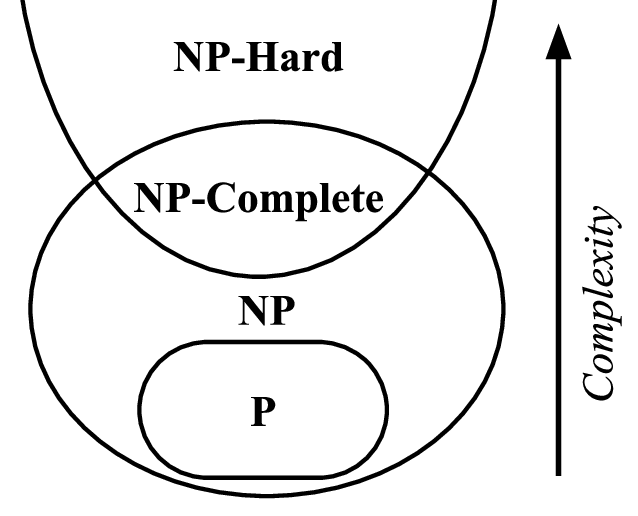
\includegraphics[width = 0.7\textwidth]{images/NP.png}
   \end{frame}

   \begin{frame}{How to solve Combinatorial optimization problem}
     \begin{itemize}
       \item Branch and bound
       \item Cutting plane
       \item Column generation
       \item ......
     \end{itemize}

   \end{frame}

   \begin{frame}{Summary}
     Finally, we should master how to settle a problem in that way, so that we will have more ideas and try different methods.

     In the process of practice,they can guarantee to find the global solution, but in solving some typical practical problems, the price is too high, or it is easy to fall into local optimum. Because it's hard to accelerate the algorithm that can guarantee to find the optimal solution, that is, for most practical problems, it is difficult to find polynomial algorithm, because most of them are NP hard problems, then the rest selection is to design an algorithm that can jump out of local optimum.
   \end{frame}
